\documentclass[12pt]{report} % You can use 'article' or 'book' class as well

\usepackage{graphicx} % For including images
\usepackage{amsmath}
\usepackage{amssymb}
\usepackage{multicol}
\usepackage{pgfplots}
\usepackage{tikz}

\begin{document}

% Title page
\begin{titlepage}
	\centering
	\vspace*{1cm} % Adjusts vertical space for the image
	% Insert your image (use the actual path and filename of your image)
	
\includegraphics[width=0.3\textwidth]{../images/KMITL Logo.png} % Adjust width as needed

	\vspace{1cm} % Vertical space after the image
	{\LARGE \textbf{Week 6 Homework}} \\[0.5cm] % Title
	\vspace{0.5cm}
	{\large \textbf{Probability Model and Data Analysis}} \\[0.5cm]
    {\large \textbf{Software Engineering Program,}} \\[0.5cm]
	{\large \textbf{Department of Computer Engineering,}} \\[0.5cm]
	{\large \textbf{School of Engineering, KMITL}} \\[1cm]
    {\Large 67011352 Theepakorn Phayonrat} \\[0.5cm] % Authors (Use \\ the separate authors)
\end{titlepage}

\section*{Homework of CDF of the discrete random variable and Bernoulli RV}

\subsection*{Question 1}

\noindent Use the CDF $F_Y[y]$ to find the following probabilities: \\

\noindent
\begin{minipage}[t]{0.55\textwidth}
\begin{tikzpicture}[baseline]
    \begin{axis}[
        width=7cm,
        height=5.5cm,
        xmin=0, xmax=5,
        ymin=0, ymax=1.1,
        axis x line=bottom,
        axis y line=left,
        xlabel={$y$},
        ylabel={$F_Y(y)$},
        ytick={0,0.2,...,1},
        xtick={0,1,2,3,4,5},
        domain=0:5,
        samples=100,
        no marks,
        clip=false
    ]
    % Piecewise CDF steps
    \addplot[blue, thick] coordinates {(0,0) (1,0) (1,0.6) (2,0.6) (2,0.8) (4,0.8) (4,1) (5,1)};
    \end{axis}
\end{tikzpicture}
\end{minipage}
\hfill
\begin{minipage}[b]{0.45\textwidth}
\begin{align*}
    &(1) \quad P[Y < 1] \quad\quad &&(2) \quad P[Y \leq 1] \\
    &(3) \quad P[Y > 2] \quad\quad &&(4) \quad P[Y \geq 2] \\
    &(5) \quad P[Y = 1] \quad\quad &&(6) \quad P[Y = 3]\\
    \\
\end{align*}
\end{minipage}

\subsection*{Solution}

\noindent From the CDF graph given earlier, we can analyse that \\

\begin{multicols}{2}
F_Y(y) =
\begin{cases}
0 & y < 1, \\
0.6 & 1 \le y < 2, \\
0.8 & 2 \le y < 4, \\
1 & y \ge 4 \\
\end{cases}

\therefore P_Y(y) =
\begin{cases}
0.6 & y = 1, \\
0.2 & y = 2, \\
0 & y = 3, \\
0.2 & y = 4, \\
0           & \text{otherwise}.
\end{cases}
\end{multicols}

\subsection*{Answer}

\noindent Therefore, we can now find the answer of the questions above.

\begin{align*}
    &(1) \quad P[Y < 1] = 0 \quad\quad &&(2) \quad P[Y \leq 1] = 0 + 0.6 = 0.6 \\
    &(3) \quad P[Y > 2]  = 0 + 0.2 = 0.2 \quad\quad &&(4) \quad P[Y \geq 2] = 0.2 + 0 + 0.2 = 0.4 \\
    &(5) \quad P[Y = 1] = 0.6 \quad\quad &&(6) \quad P[Y = 3] = 0 \\
\end{align*}

\newpage

\subsection*{Question 2}

\noindent Flip a coin and let it land on the table, then observe
whether head or tail facing up after the coin lands. The event of the
head facing up is considered as a success while the event of tail
facing up is considered as failure. \\

\noindent Let $X$ be the random variable of the success event. \\
1. Find and sketch the PMF of $X$. \\
2. Find the expected value of $E[X]$ \\\
3. Find and sketch the CDF of $X$. \\

\subsection*{Answer}

\begin{multicols}{2}
\[
P_X(x) =
\begin{cases}
0.5 & x = 0, \\
0.5 & x = 1, \\
0 & \text{otherwise}.
\end{cases}
\]
\columnbreak
\\
\begin{center}
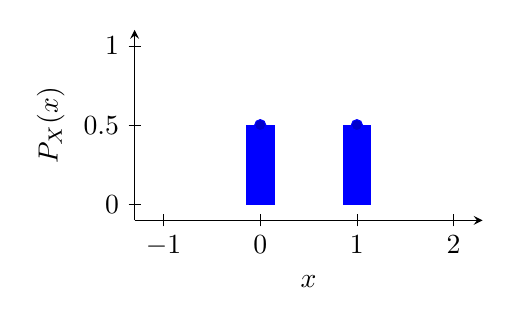
\begin{tikzpicture}
\begin{axis}[
    ymin=0, ymax=1,
    xmin=-1, xmax=2,
    xtick={-1,0,1,2},
    ytick={0,0.5,1},
    axis lines=left,
    width=6cm,
    height=4cm,
    enlargelimits=0.1,
    ylabel={$P_X(x)$},
    xlabel={$x$},
    tick style={black},
    ymajorgrids=false,
    xmajorgrids=false,
    every axis plot/.append style={ybar, bar width=10pt, black, fill=black}
]
\addplot coordinates {(0,0.5) (1,0.5)};
\end{axis}
\end{tikzpicture}
\end{center}
\end{multicols}

\noindent $\therefore E[X] = P[X = 0](0) + P[X = 1](1) = 0.5(0) + 0.5(1) = 0 + 0.5 = 0.5$

\begin{multicols}{2}
\[
F_X(x) =
\begin{cases}
0 & x < 0, \\
0.5 & 0 \le x < 1, \\
1 & x \ge 1 \\
\end{cases}
\]
\columnbreak
\\
\begin{tikzpicture}
    \begin{axis}[
        width=6cm,
        height=4cm,
        xmin=-1, xmax=2,
        ymin=0, ymax=1,
        axis x line=bottom,
        axis y line=left,
        xlabel={$x$},
        ylabel={$F_X(x)$},
        ytick={0,0.5,1},
        xtick={-1,0,1,2},
        domain=0:5,
        samples=100,
        no marks,
        clip=false
    ]
    \addplot[blue, thick] coordinates {(-1,0) (0,0) (0,0.5) (1,0.5) (1,1) (2,1)};
    \end{axis}
\end{tikzpicture}
\end{multicols}

\end{document}
